\documentclass[11pt]{article}

\usepackage{amsmath, amssymb, amsthm}
\usepackage{tikz}

\theoremstyle{plain}
\newtheorem{thm}{Theorem}[section]
\newtheorem*{thm*}{Theorem}
\newtheorem{prop}[thm]{Proposition}
\newtheorem{lem}[thm]{Lemma}
\newtheorem*{lem*}{Lemma}
\newtheorem{dfn}[thm]{Definition}
\newtheorem{cor}[thm]{Corollary}
\newtheorem{claim}[thm]{Claim}
\newtheorem{conj}[thm]{Conjecture}
\newtheorem{ques}[thm]{Question}
\newtheorem*{rem}{Remark}


\oddsidemargin  0pt
\evensidemargin 0pt
\marginparwidth 40pt
\marginparsep 10pt
\topmargin 0pt
\headsep 10pt
\textheight 8.2in
\textwidth 6.4in
\renewcommand{\baselinestretch}{1.1}

\newcommand{\codeg}{\text{codeg}}
\newcommand{\BBE}{\mathbb{E}}
\newcommand{\BFP}{\mathbf{P}}
\usepackage{amsmath}
\usepackage{amsthm}
\usepackage{amssymb}
\usepackage{mathtools}
\usepackage{hyperref}
\usepackage{url}





\usepackage{graphicx}
\usepackage{caption}
\usepackage{subcaption}

\def\eQb#1\eQe{\begin{eqnarray*}#1\end{eqnarray*}}
\def\eQnb#1\eQne{\begin{eqnarray}#1\end{eqnarray}}
\providecommand{\e}[1]{\ensuremath{\times 10^{#1}}}
\providecommand{\pb}[0]{\pagebreak}
\DeclarePairedDelimiter\ceil{\lceil}{\rceil}
\DeclarePairedDelimiter\floor{\lfloor}{\rfloor}

\newcommand{\E}{\mathrm{E}}
\newcommand{\Var}{\mathrm{Var}}
\newcommand{\Cov}{\mathrm{Cov}}

\def\Qb#1\Qe{\begin{question}#1\end{question}}
\def\Sb#1\Se{\begin{solution}#1\end{solution}}


\newtheoremstyle{quest}{\topsep}{\topsep}{}{}{\bfseries}{}{ }{\thmname{#1}\thmnote{ #3}.}
\theoremstyle{quest}
\newtheorem*{definition}{Definition}
\newtheorem*{theorem}{Theorem}
\newtheorem*{lemma}{Lemma}
\newtheorem*{question}{Question}
\newtheorem*{preposition}{Preposition}
\newtheorem*{exercise}{Exercise}
\newtheorem*{challengeproblem}{Challenge Problem}
\newtheorem*{solution}{Solution}
\newtheorem*{remark}{Remark}
\usepackage{verbatimbox}
\usepackage{listings}
\usepackage{mathrsfs}
\date{}
\title{\vspace{-0.7cm}
Limit Theorems II: Final}

\author{
Youngduck Choi 
\thanks{Department of Mathematics, Courant Institute of Mathematical Sciences, 
yc1104@nyu.edu; If you find an error and want to share with me, 
you can reach me via email.
}}

\begin{document}

\maketitle

\begin{abstract}
This work contains solutions for the final of the Limit Theorems II by Professor
McKean.
\end{abstract}


\begin{question}[1-1]
\hfill
\begin{figure}[h!]
  \centering
    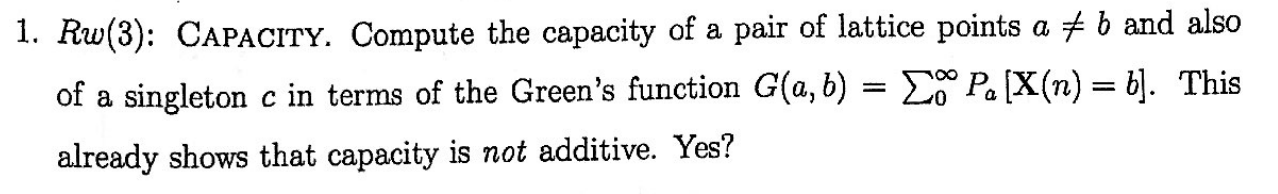
\includegraphics[width=0.7\textwidth]{limthm2-f-p1.png}
\end{figure}
\end{question}
\begin{solution} \hfill \\
\end{solution}

\newpage

\begin{question}[1-2]
\hfill
\begin{figure}[h!]
  \centering
    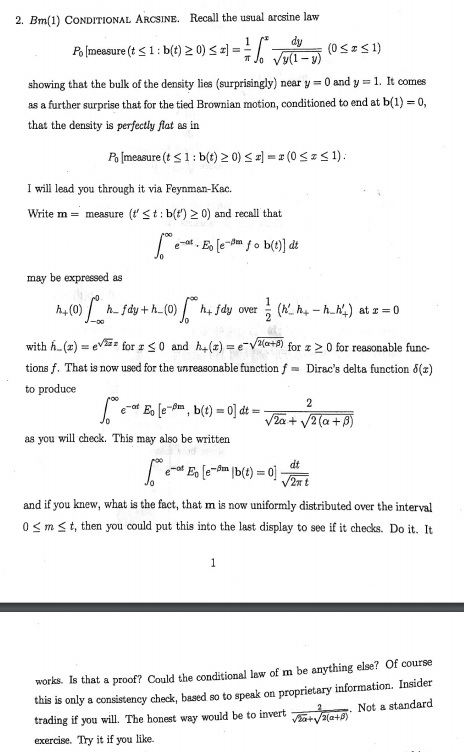
\includegraphics[width=0.7\textwidth]{limthm2-f-p2.png}
\end{figure}
\end{question}
\begin{solution} \hfill \\
\end{solution}

\newpage

\begin{question}[1-3]
\hfill
\begin{figure}[h!]
  \centering
    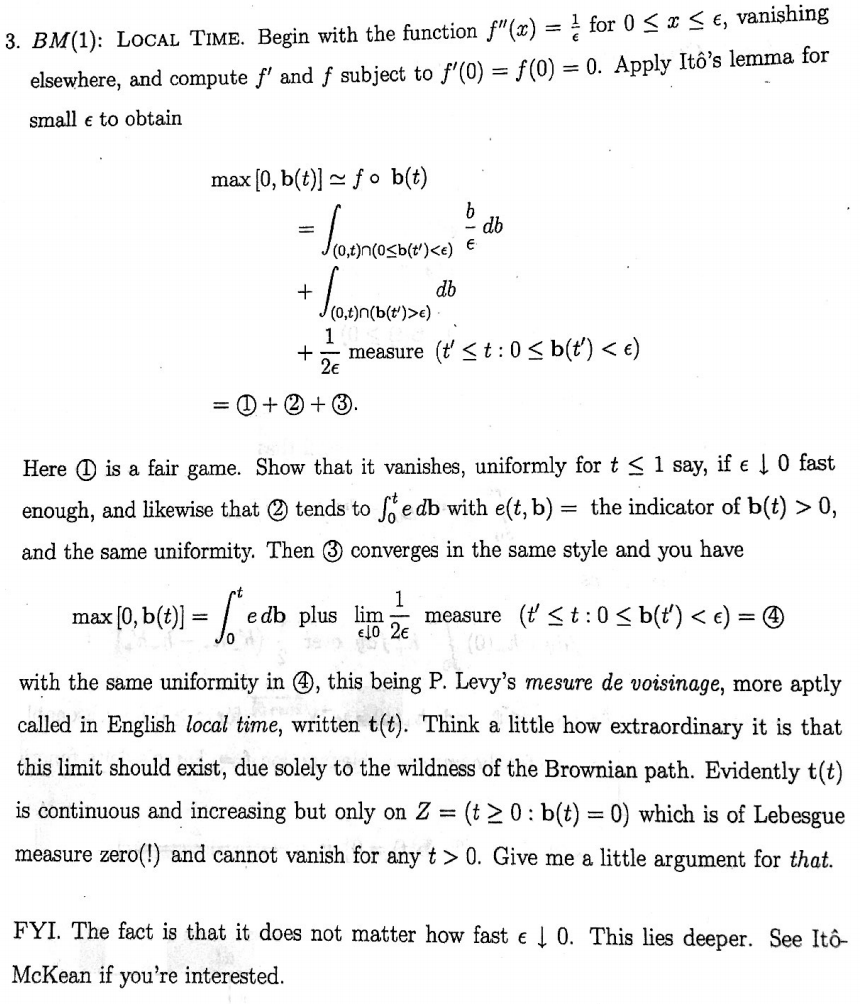
\includegraphics[width=0.7\textwidth]{limthm2-f-p3.png}
\end{figure}
\end{question}
\begin{solution} \hfill \\
Recall the Ito's formula for single martingales: If $f$ is $C^2$ and for all $0 \leq t$,
\eQb
E\int_{0}^{t} [f'(M(s))]^2 dA(s) < \infty \>\>\> &\text{and}& \>\>\> E\int_{0}^{t} 
|f''(M(s))|dA(s) < \infty
\eQe
then, for all $0 \leq t$,
\eQnb
f(M(t)) - f(M(0)) &=& \int_{0}^{t} f'(M(s)) dM(s) + \dfrac{1}{2} \int_{0}^{t} 
f'(M(s)) dA(s) \label{eq:1-3-1}
\eQne
where $A(t)$ is the unique increasing, continuous process, corresponding to $M(t)$.
Of course, for the problem at hand, we have $M(t) = B(t)$ and $A(t) = t$, so $db(s)$ and
$ds$ will be used to denote the integrators. 
Now, to compute local time, we cannot naively apply this formula, as $\max(0,\cdot)$ is 
not $C^2(\mathbb{R})$. Hence, we approximate with the suggested strategy. 
Let $f_{\epsilon}$ be defined as given for each $\epsilon > 0$. Then, 
for any $0 \leq t$, and $\epsilon > 0$,
\eQnb
f_{\epsilon} \circ b(t) &=& f_{\epsilon} \circ b(t) - f_{\epsilon} \circ b(0) 
= \int_{0}^{t} f_{\epsilon}^{'}(B(s)) db(s) + \dfrac{1}{2} \int_{0}^{t}  
f_{\epsilon}^{''} (B(s)) ds \label{eq:1-3-2} \\ 
&=& \int_{\{s \in [0,t] : 0 \leq b(s) < \epsilon\}} \dfrac{b(s) }{\epsilon} db(s)
+ \int_{\{s \in [0,t] : b(s) > \epsilon\}} 1 db(s)
+ \dfrac{1}{2} \int_{ \{s \in [0,t] : 0 \leq b(s) < \epsilon\} } \dfrac{1}{\epsilon} 
ds  \label{eq:1-3-3} \\
&=& 
\int_{\{s \in [0,t] : 0 \leq b(s) < \epsilon\}} \dfrac{b(s) }{\epsilon} db(s)
+ \int_{\{s \in [0,t] : b(s) > \epsilon\}} 1 db(s) \nonumber 
+ \dfrac{1}{2\epsilon} \lambda_1( \{ s \in [0,t] : 0 \leq b(s) < \epsilon \}) \nonumber
\\ 
&=:& (I) + (II) + (III) \nonumber 
\eQne 
where~\eqref{eq:1-3-2} follows from~\eqref{eq:1-3-1},~\eqref{eq:1-3-3} follows
from definition of $f_{\epsilon}$ for each $\epsilon > 0$, and $\lambda_1$ denotes
1-dimensional Lebesgue measure as hinted. With the given fact that $(I)$ is a 
martingale, we claim that, for any $0 \leq t \leq 1$ uniformly, 
\eQnb
\int_{\{s \in [0,t] : 0 \leq b(s) < \epsilon\}} \dfrac{b(s)}{\epsilon} db(s) \>\>\> 
\text{converges to} \>\> 0 \label{eq:1-3-4}
\eQne
and
\eQnb
\int_{\{s \in [0,t] :  b(s) > \epsilon \}} 1 db(s) \>\>\> 
\text{converges to} \int_{0}^{t} e(s)  db(s)
\label{eq:1-3-5} 
\eQne
as $\epsilon \downarrow 0$ $\mathbb{P}$ almost surely, so that 
\eQb
\max(0,b(t)) = \int_{0}^{t} e(s) db(s) + \lim_{\epsilon \downarrow 0} \dfrac{1}{2
\epsilon} \lambda_1( \{s \in [0,t] : 0 \leq b(s) < \epsilon\}) \>\>\> \textbf{P} \>\>\>
\text{almost surely}  
\eQe 
where the last limit exists, since for any  $\mathbb{P}$-a.s. $\omega \in \Omega$, 
$0 \leq t \leq 1$,
\eQb
\lambda_1( \{s \in [0,t] : 0 \leq b(s)(w) < \epsilon\}). 
\eQe 
Then, for each $0 \leq t \leq 1$, for some
universal constant $C$, independent of $t$,
\eQnb
E\left[ \int_{0}^{t} \dfrac{b(s)}{\epsilon} 1_{\{0 \leq b(s) < \epsilon\}} - 0 db(s) 
\right]^2 
&=& E \int_{0}^{t} \left[ 
\dfrac{b(s)}{\epsilon} 1_{\{0 \leq b(s) < \epsilon\}} \right]^2 ds \label{eq:1-3-6} \\
&\leq& E \int_{0}^{t} 1_{\{ 0 \leq b(s) < \epsilon\}} ds \nonumber \\
&=& \int_{0}^{t} P(0 \leq b(s) < \epsilon) ds \nonumber \\
&=& \int_{0}^{t} P(0 \leq b(1) < \dfrac{\epsilon}{\sqrt{s}}) ds \label{eq:1-3-7} \\
&\leq& \int_{0}^{t} P(|b(1)| < \dfrac{\epsilon}{\sqrt{s}}) ds \leq C\sqrt{t} \epsilon
\label{eq:1-3-8},
\eQne
where~\eqref{eq:1-3-6} holds by the Ito $L^2$ isometry,~\eqref{eq:1-3-7} follows by 
the scaling of BW(1), and~\eqref{eq:1-3-8} follows from the fact that  
\eQb
\dfrac{P(|b(1) \leq x)}{x} \>\>\> \text{is uniformly bounded } \>\>\> \text{for all} 
\>\>\> x > 0. 
\eQe
Hence, if $\epsilon = \Omega(n^2)$, then, by Doob's inequality,
\eQb
(I) \to 0 \>\>\> \text{uniformly for } \>\>\> 0 \leq t \leq 1 \>\>\> P \>\>\> 
\text{almost surely}
\eQe
showing~\eqref{eq:1-3-4}.

Now, from uniformity of convergence and continuity of Lebesgue measure, we see that
$\textbf{t}(t)$ is continuous, and clearly increasing as (II) and (III) are
increasing in t almost surely. 
 
\end{solution}

\newpage

\begin{question}[1-4]
\hfill
\begin{figure}[h!]
  \centering
    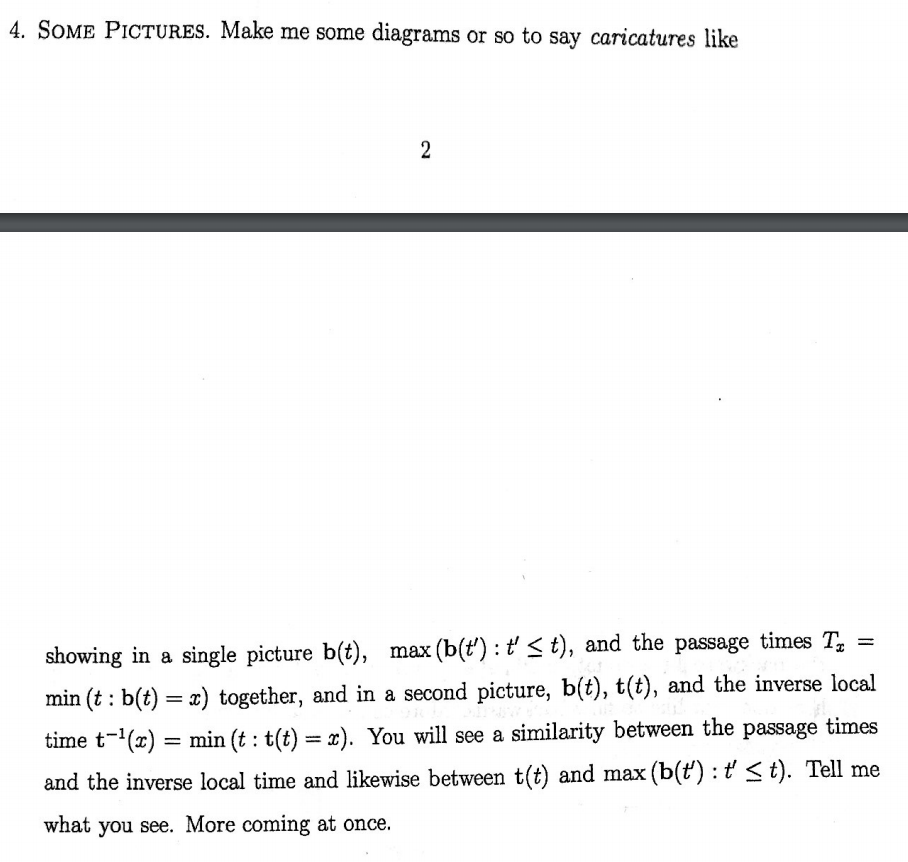
\includegraphics[width=0.7\textwidth]{limthm2-f-p4.png}
\end{figure}
\end{question}
\begin{solution} \hfill \\
\end{solution}

\newpage

\begin{question}[1-5]
\hfill
\begin{figure}[h!]
  \centering
    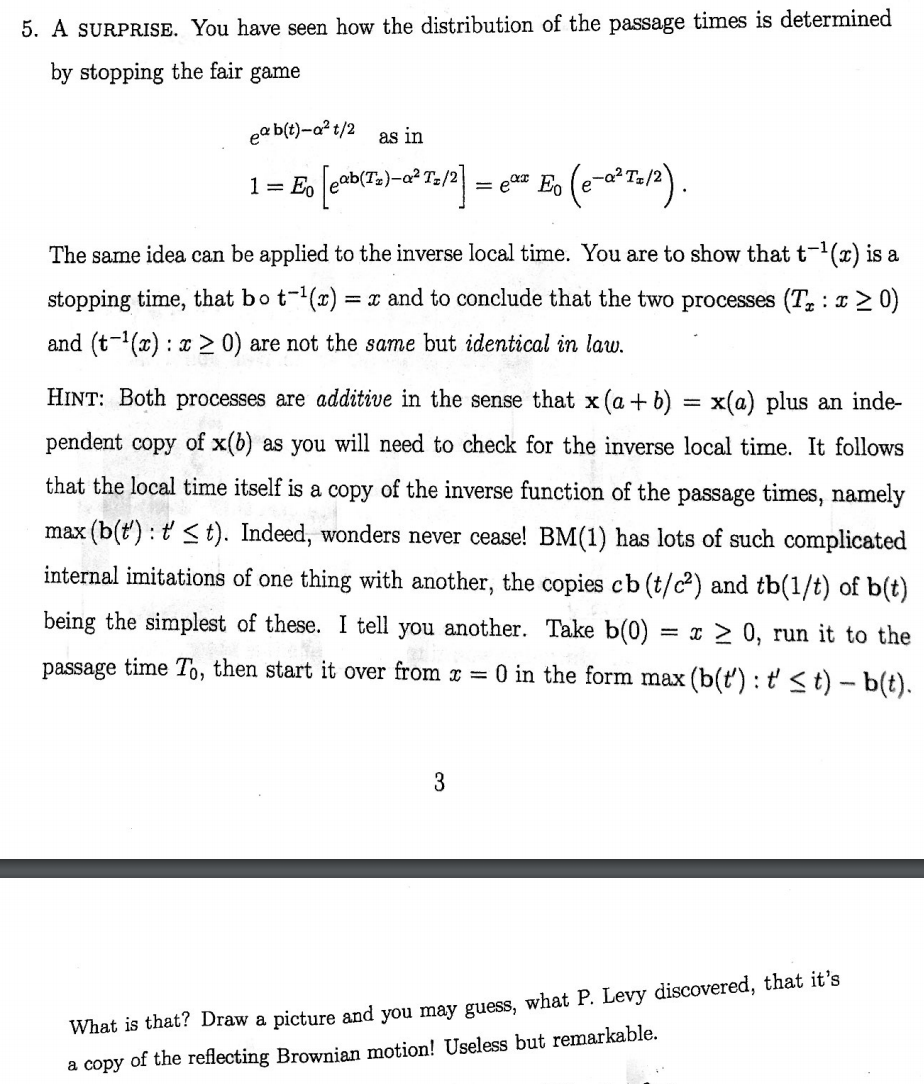
\includegraphics[width=0.7\textwidth]{limthm2-f-p5.png}
\end{figure}
\end{question}
\begin{solution} \hfill \\
\end{solution}

\newpage

\begin{question}[1-6]
\hfill
\begin{figure}[h!]
  \centering
    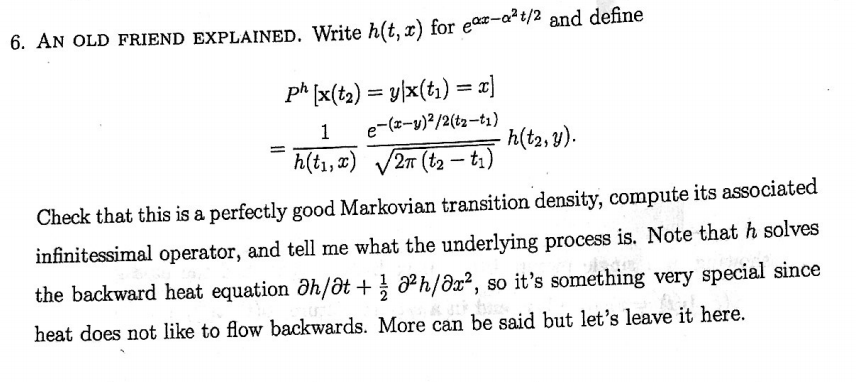
\includegraphics[width=0.7\textwidth]{limthm2-f-p6.png}
\end{figure}
\end{question}
\begin{solution} \hfill \\
We check that $P^h$ is a Markovian transition density by checking that it integrates
to 1 with respect to $y$. We compute, via completing the square,
\eQb
\int P^h(\bold{x}(t_2) = y | \bold{x}(t_1) = x) dy &=& \int
\dfrac{h(t_2,y)}{h(t_1,x)} 
\dfrac{e^{-(x-y)^2/2(t_2 - t_1)}}{\sqrt{2\pi(t_2 - t_1)}} dy \\
&=& \dfrac{1}{h(t_1,x)} \dfrac{1}{\sqrt{2\pi(t_2 -t_1)}} \int e^{-(y^2 - 2xy +x^2)/
2(t_2 - t_1) + \alpha y - \alpha^2 t_2/2} dy  \\
&=& \dfrac{1}{h(t_1,x)} e^{\alpha x - \frac{1}{2} \alpha^2 t_1} \int 
e^{\frac{-(y - (x + \alpha(t_2 - t_1))^2}{2(t_2 - t_1)}} dy  \\
&=& \dfrac{1}{h(t_1,x)} e^{\alpha x - \frac{1}{2} \alpha^2 t_1} = \dfrac{h(t_1,x)}{
h(t_1,x)} = 1.
\eQe
Now, we compute the associated infinitessimal operator. From the general theory, we 
know that the generator must be defined by
\eQnb
\mathscr{G}(t_1) f(x) &=& \lim_{t_2 \downarrow t_1} \dfrac{\int f(y)P^h(
\bold{x}(t_2) = y | \bold{x}(t_1) = x) dy - f(x)}{t_2 - t_1} \\
\eQne
whenever the limit is well-defined for $f \in C_0(\mathbb{R})$.

By observing that $h$ satisfies the backward heat equation, we further compute
for each $0 \leq t$,
\eQb
\mathscr{G}(t)f &=& \dfrac{1}{h} \partial_t h f + \dfrac{1}{2} \partial_x (f_x h 
+ h_X f) \\
&=& \dfrac{1}{h} \partial_{t} h f + \dfrac{1}{2h} (f_{xx} h + 2 f_x h_x + h_{xx} f) \\
&=& \dfrac{1}{2} 
\eQe
\end{solution}
\end{document}
